\section{Signal generators}
\subsection{Bistable circuits - Schmitt trigger}
\subsubsection*{Generic bistable circuit - schmitt trigger}
A generic bistable circuit, called also schmitt trigger is a circuit that has two stable states and can remain in either state
indefinitely until an external trigger is applied to change its state. 

It can be made of an op amp with positive feedback (no virtual ground). When the circuit turns on, \(V_{out}\), \(V_+\) and
\(V_-\) are initially at \(0 \; V\). A slight variation in the input voltage \(V_+\) will cause the output to saturate at either
\(L_+\) or \(L_-\) depending on the sign of the variation. These two final states are the two stable states of the circuit.
Due to the positive feedback, the circuit will remain in the stable state until an external trigger is applied to one of the
input terminals.

\begin{center}
	\begin{circuitikz}[american, scale=0.8, transform shape]
		\draw (0,0) node[op amp, yscale=-1] (opamp) {};
		\node[ground] at (opamp.-) {}; 
		\node[left] at (opamp.+) {\(V_+\)};
		\draw (opamp.+) -- ++(0,1);
		\draw (opamp.out) to[short, -o] ++(0.5,0) node[right] {\(V_{out}\)};
		\draw (opamp.out) -- ++(0, 1.5)
			to[R, l=\(R_2\)] ++(-2.5, 0)
			to[R, l=\(R_1\)] ++(-2, 0) node[ground] {};
	\end{circuitikz}
\end{center}

\subsubsection*{Inverting bistable circuit}
An inverting bistable circuit is a Schmitt trigger with a voltage generator (that acts as a trigger) connected to the inverting
input of the op amp. It is called ``inverting'' because the output voltage is inverted with respect to the input trigger voltage. 

The output voltage \(V_{out}\) will be at \(L_+\) and \(V_+ = L_+ \cdot R_1 / (R_1 + R_2)\) until the input trigger voltage
\(V_{in}\) exceeds the positive threshold voltage \(V_{TH} = L_+ \cdot R_1 / (R_1 + R_2)\). In this case the differential input
voltage becomes negative (\(V_+ - V_{in} < 0\)), the output voltage \(V_{out}\) will switch to \(L_-\) and
\(V_+ = L_- \cdot R_1 / (R_1 + R_2)\).

To switch back to \(L_+\), the input trigger voltage \(V_{in}\) must be lower than the negative threshold voltage
\(V_{TL} = L_- \cdot R_1 / (R_1 + R_2)\). In this case the differential input voltage become positive again
(\(V_+ - V_{in} > 0\)) to switch the output back to \(L_+\).

\[V_{out} = L_+ \quad \Longleftrightarrow \quad V_+ - V_{in} = L_+ \cdot \frac{R_1}{R_1 + R_2} - V_{in} > 0 \quad \Longrightarrow \quad V_{in} < V_{TH} = L_+ \cdot \frac{R_1}{R_1 + R_2}\]
\[V_{out} = L_- \quad \Longleftrightarrow \quad V_+ - V_{in} = L_- \cdot \frac{R_1}{R_1 + R_2} - V_{in} < 0 \quad \Longrightarrow \quad V_{in} > V_{TL} = L_- \cdot \frac{R_1}{R_1 + R_2}\]

\begin{center}
	\begin{minipage}{0.45\textwidth}
		\centering \begin{circuitikz}[american, scale=0.8, transform shape]
			\draw (0,0) node[op amp, yscale=-1] (opamp) {};
			\node[left] at (opamp.+) {\(V_+\)};
			\draw (opamp.+) -- ++(0,1);
			\draw (opamp.out) to[short, -o] ++(0.5,0) node[right] {\(V_{out}\)};
			\draw (opamp.out) -- ++(0, 1.5)
			to[R, l=\(R_2\)] ++(-2.5, 0)
			to[R, l=\(R_1\)] ++(-2, 0) node[ground] {};
			\draw (opamp.-) -- ++(-0.5, 0) to[vsource, l_=\(V_{in}\)] ++(0, -1.5) ++(0, 0.3) node[ground] {};
		\end{circuitikz}
	\end{minipage}
	\begin{minipage}{0.45\textwidth}
		\centering 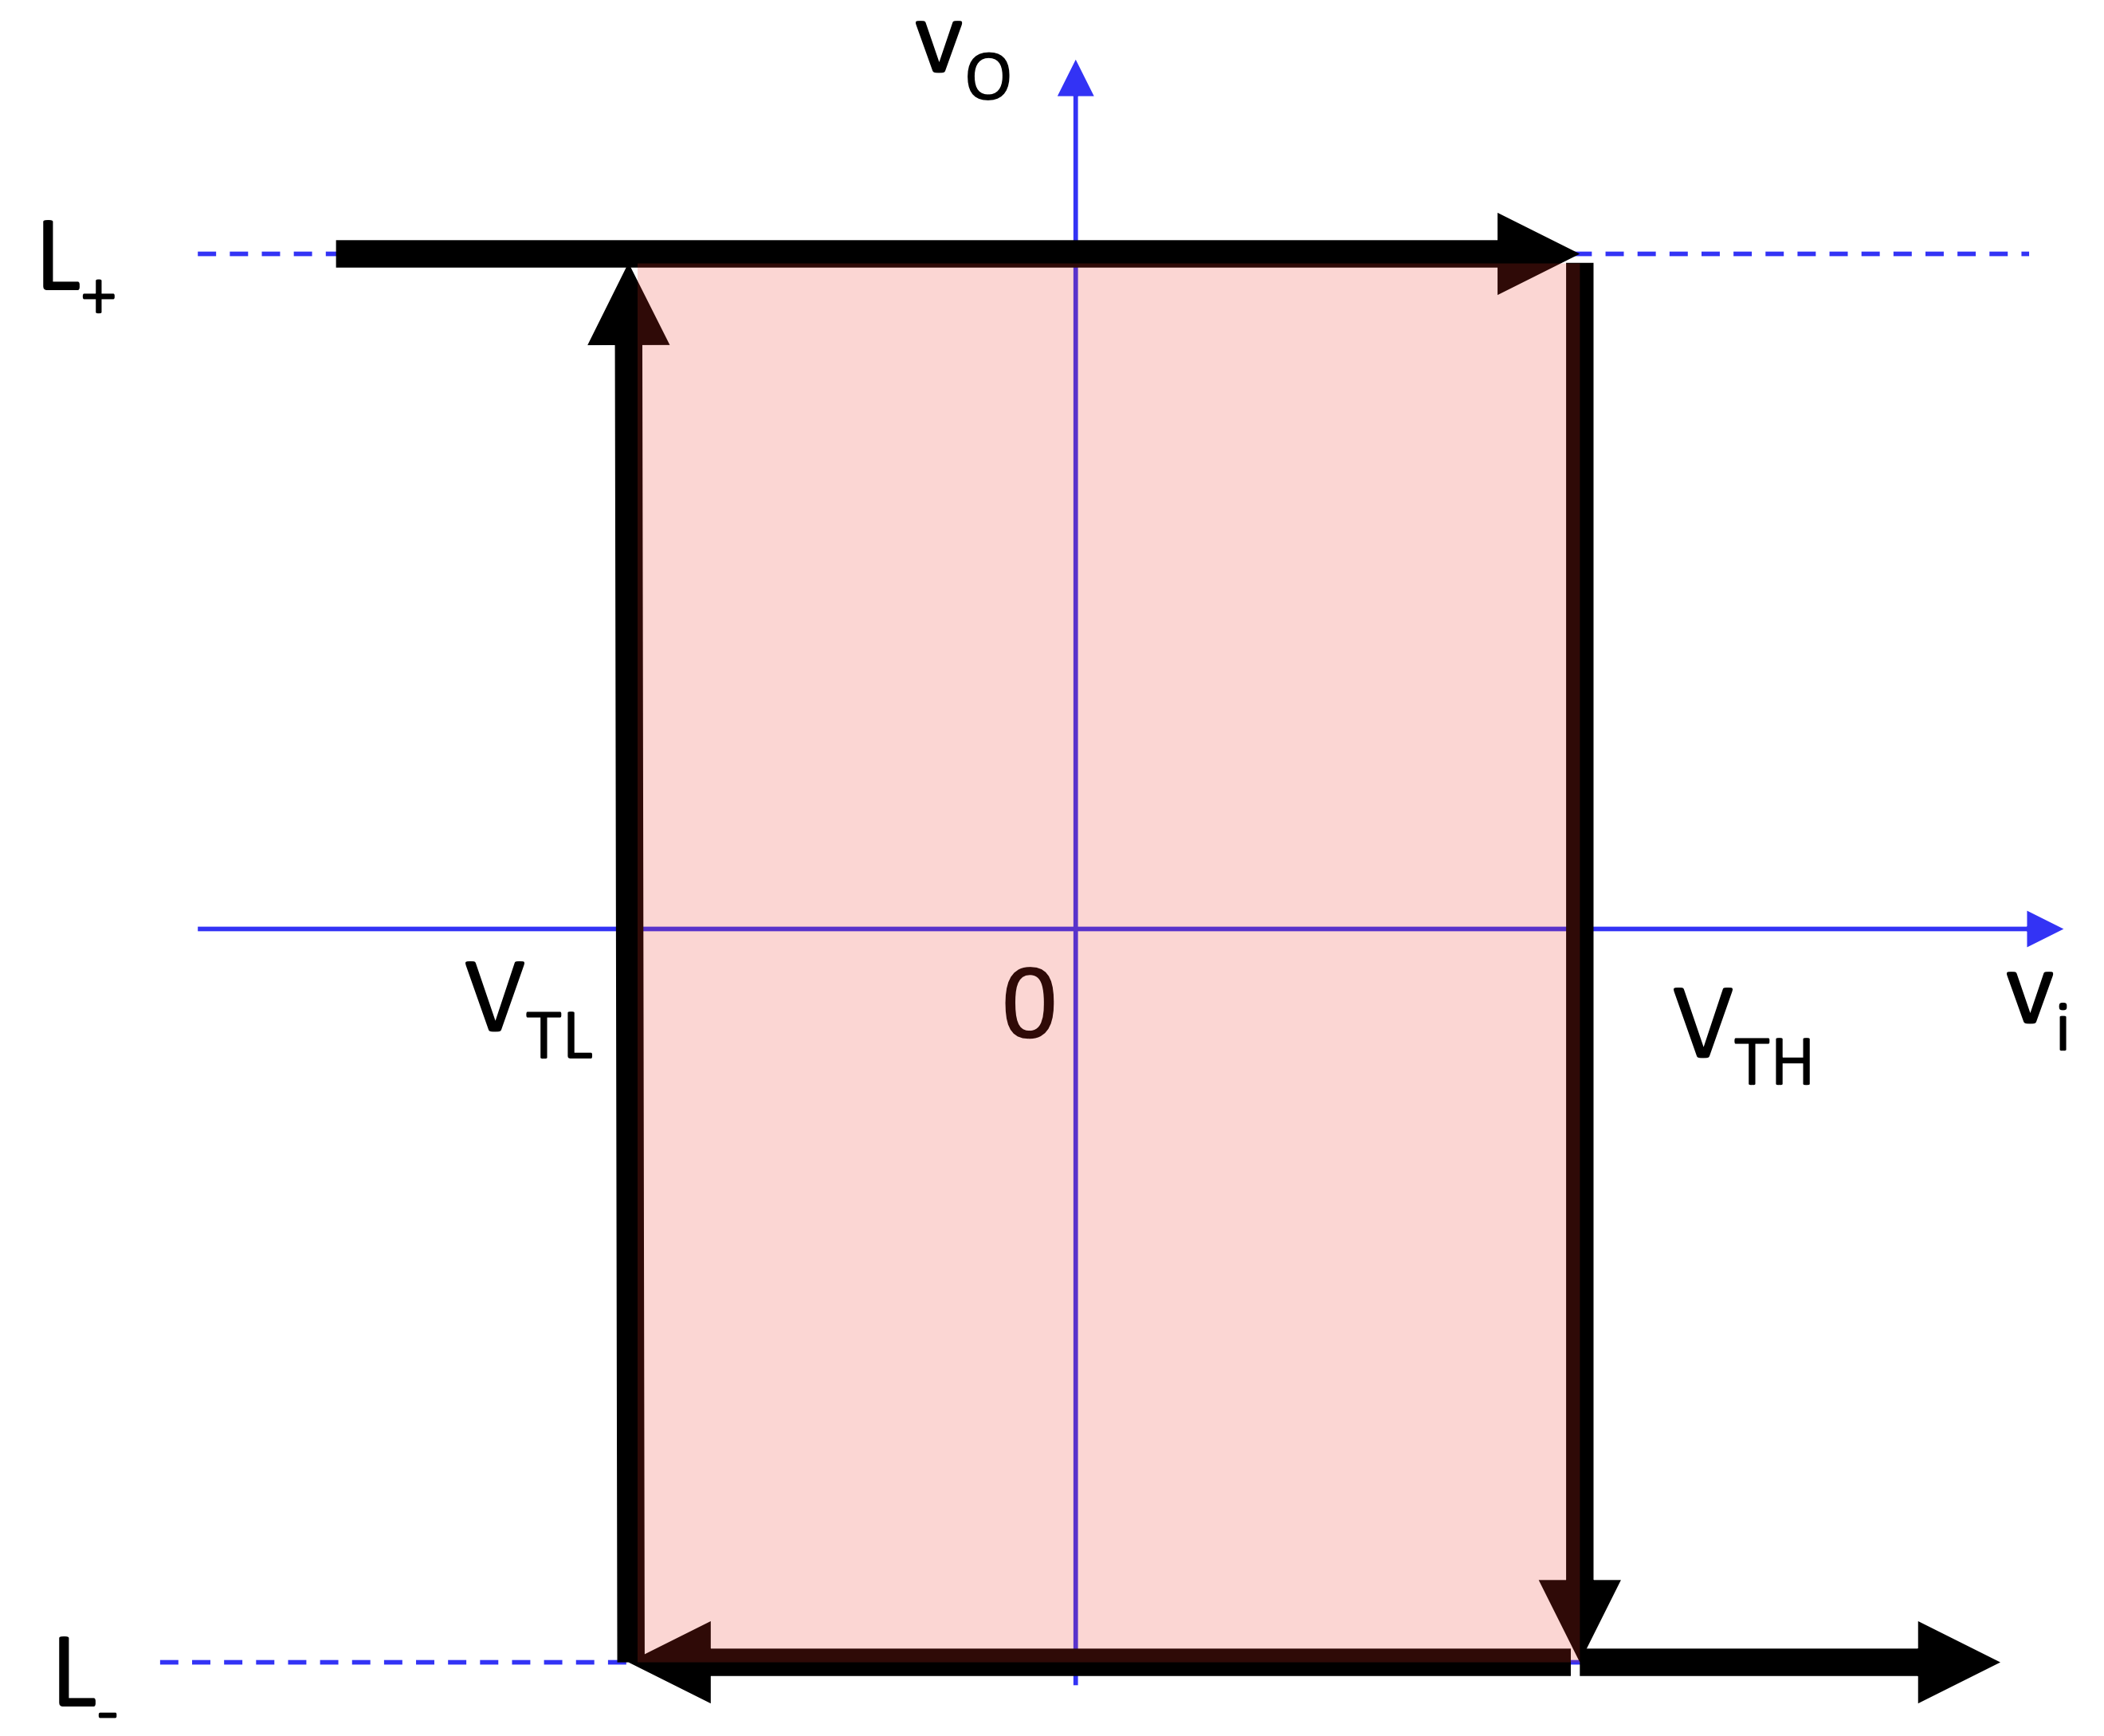
\includegraphics[width=0.7\textwidth]{immagini/inverting_bistable.png}
	\end{minipage}
\end{center}

\newpage

\subsubsection*{Non inverting bistable circuit}
A non inverting bistable circuit is a Schmitt trigger with a voltage generator (that acts as a trigger) connected at the end of
the voltage divider that feeds the non inverting input input of the op amp. It is called ``non inverting'' because the output
voltage is not inverted with respect to the input trigger voltage. 

The output voltage \(V_{out}\) will be at \(L_+\) and \(V_+ = L_+ \cdot R_1 / (R_1 + R_2) + V_{in} \cdot R_2 / (R_1 + R_2)\)
until the input trigger voltage \(V_{in}\) exceeds the negative threshold voltage \(V_{TL} = - L_+ \cdot R_1 / R_2\).
In this case the non-inverting input voltage \(V_+\) becomes negative, the output voltage \(V_{out}\) will switch to \(L_-\)
and \(V_+ = L_- \cdot R_1 / (R_1 + R_2) + V_{in} \cdot R_2 / (R_1 + R_2)\).

To switch back to \(L_+\), the input trigger voltage \(V_{in}\) must be bigger than the positive threshold voltage
\(V_{TH} = - L_- \cdot R_1 / R_2\). In this case the non inverting input voltage \(V_+\) become positive again to switch
the output back to \(L_+\).

\[V_{out} = L_+ \quad \Longleftrightarrow \quad V_+ = L_+ \cdot \frac{R_1}{R_1 + R_2} + V_{in} \cdot \frac{R_2}{R_1 + R_2} > 0 \quad \Longrightarrow \quad V_{in} > V_{TL} = -L_+ \cdot \frac{R_1}{R_2}\]
\[V_{out} = L_- \quad \Longleftrightarrow \quad V_+ = L_- \cdot \frac{R_1}{R_1 + R_2} + V_{in} \cdot \frac{R_2}{R_1 + R_2} < 0 \quad \Longrightarrow \quad V_{in} < V_{TH} = -L_- \cdot \frac{R_1}{R_2}\]

\begin{center}
	\begin{minipage}{0.45\textwidth}
		\centering \begin{circuitikz}[american, scale=0.8, transform shape]
			\draw (0,0) node[op amp, yscale=-1] (opamp) {};
			\node[ground] at (opamp.-) {}; 
			\node[left] at (opamp.+) {\(V_+\)};
			\draw (opamp.+) -- ++(0,1);
			\draw (opamp.out) to[short, -o] ++(0.5,0) node[right] {\(V_{out}\)};
			\draw (opamp.out) -- ++(0, 1.5)
			to[R, l=\(R_2\)] ++(-2.5, 0)
			to[R, l=\(R_1\)] ++(-2, 0) -- ++(-0.2,0)
			to[vsource, l_=\(V_{in}\)] ++(0, -1.5) ++(0, 0.3) node[ground] {};
		\end{circuitikz}
	\end{minipage}
	\begin{minipage}{0.45\textwidth}
		\centering 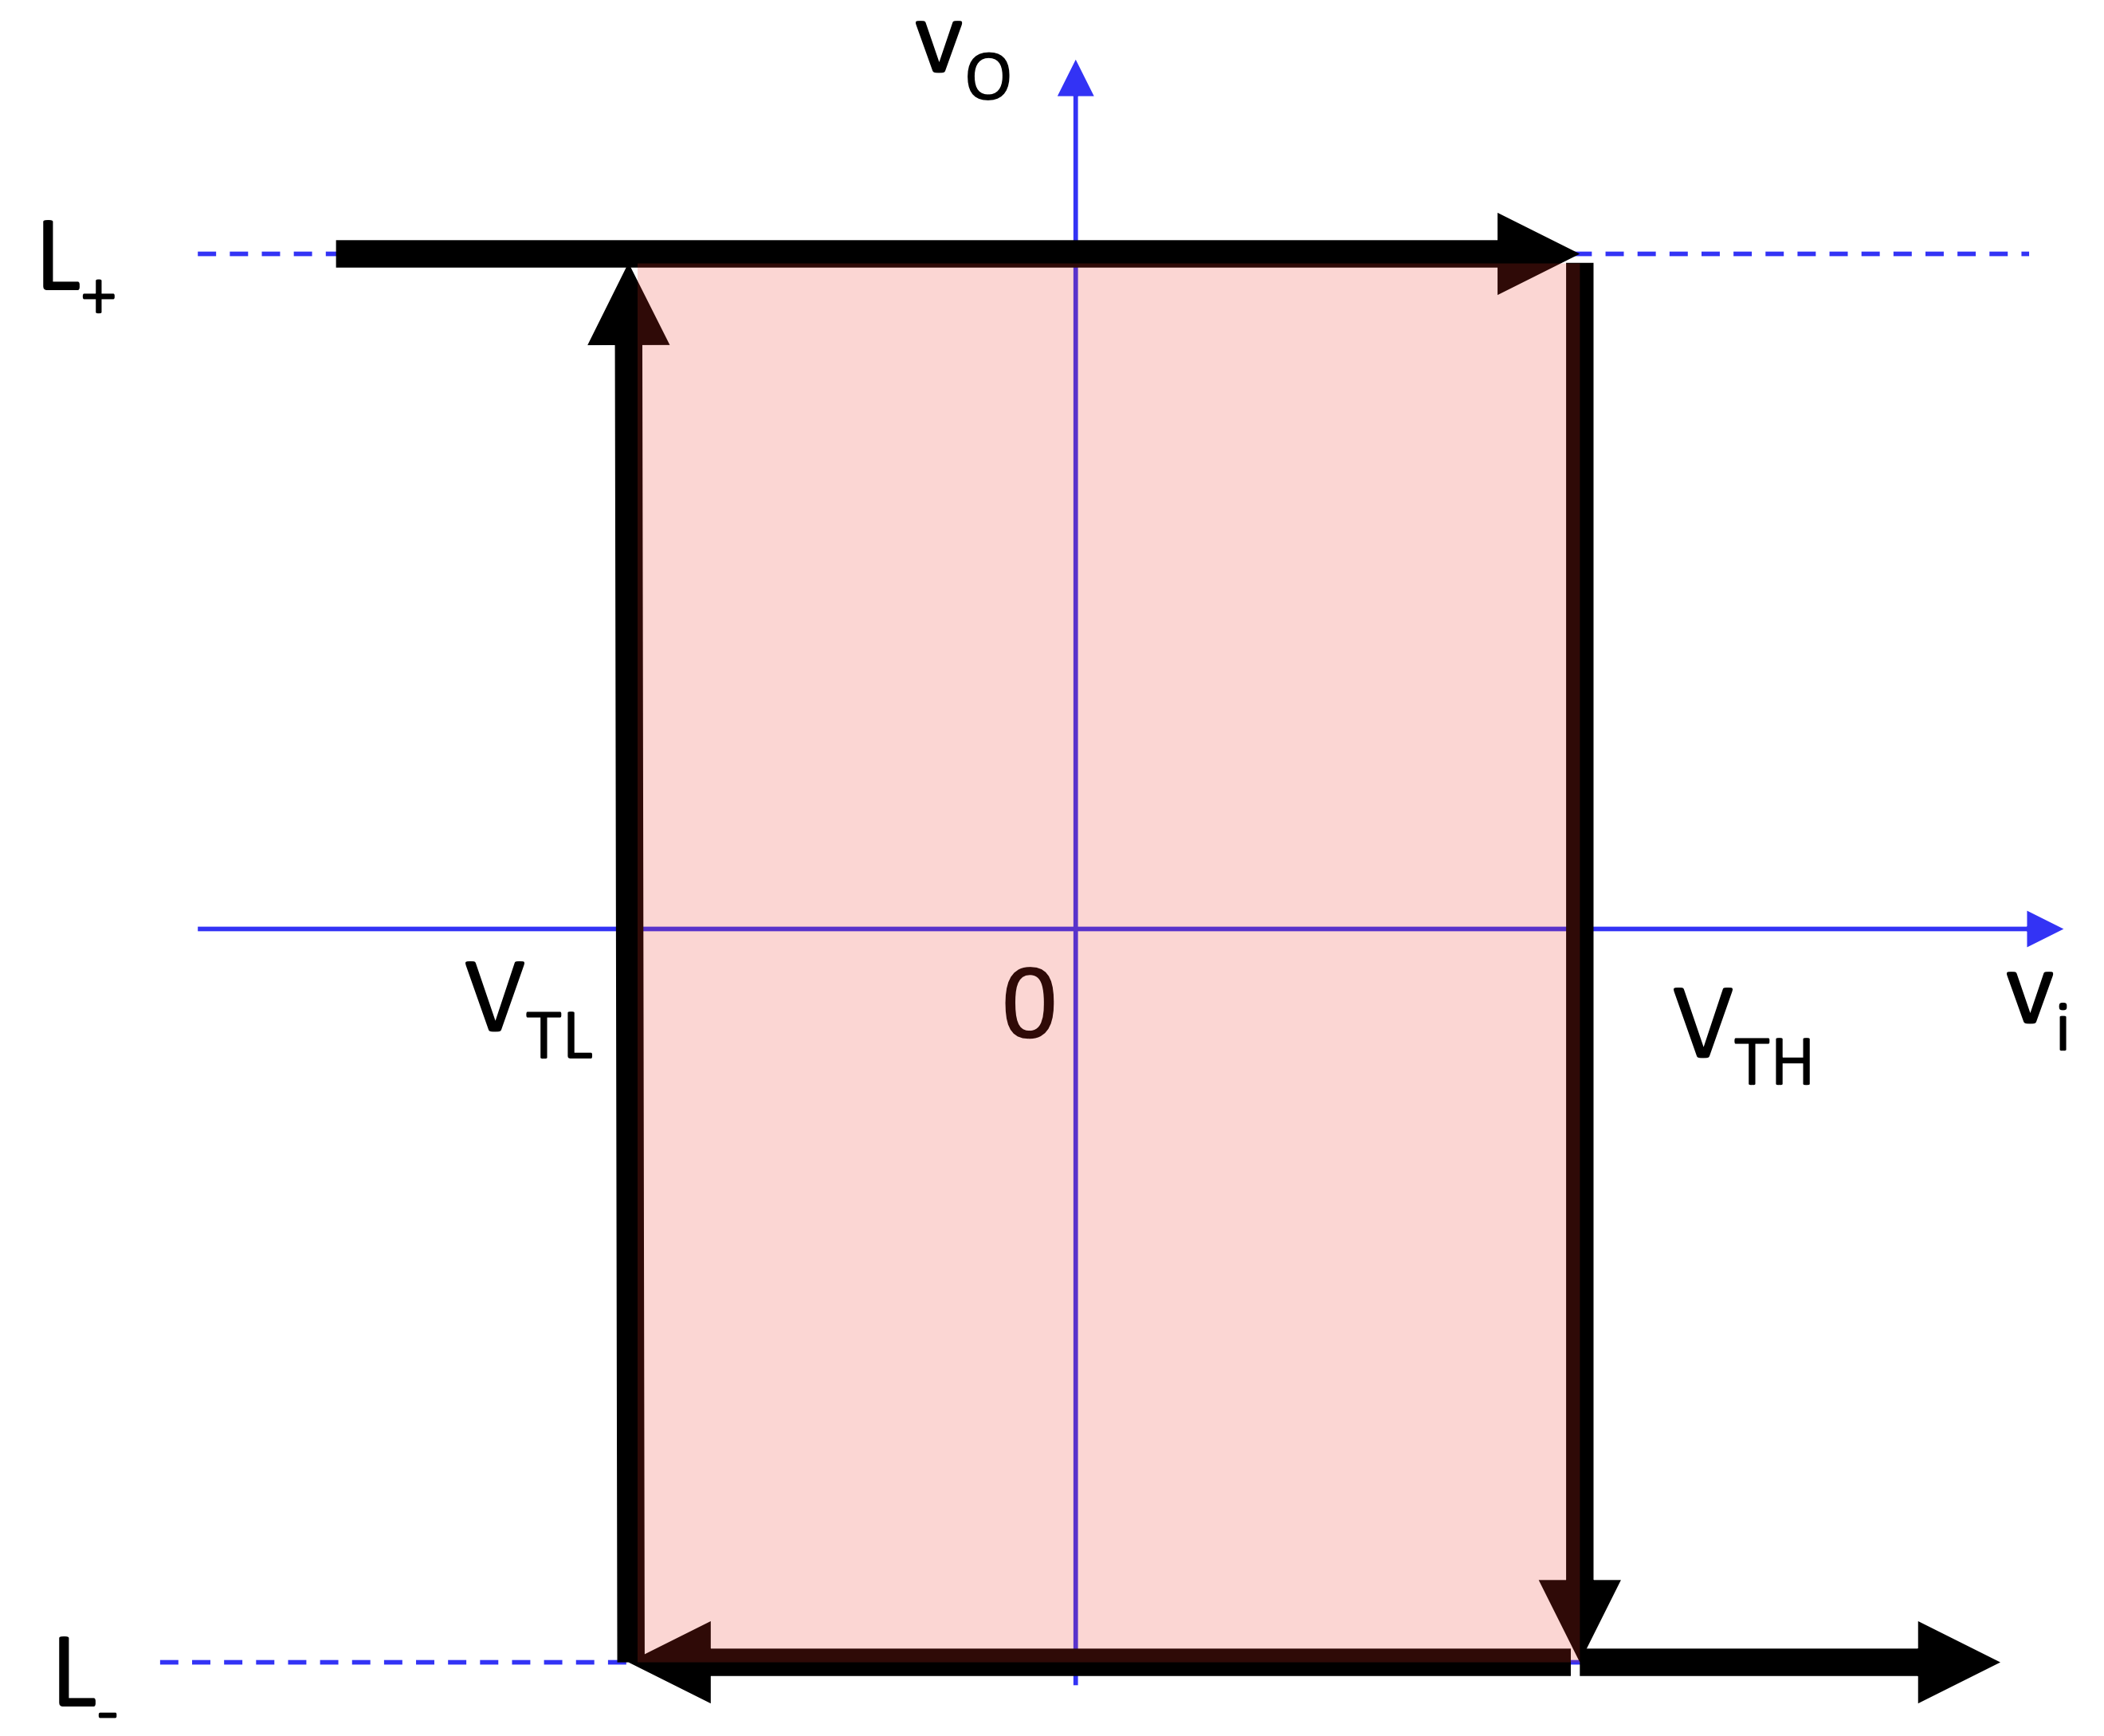
\includegraphics[width=0.7\textwidth]{immagini/inverting_bistable.png}
	\end{minipage}
\end{center}

\subsubsection*{Bistable circuit as a comparator}
The comparator is a circuit that compares two voltages and outputs a digital signal (high or low) depending on which voltage is
higher. Comparators can have hysteresis cycles (to mitigate the noise in input signal) and can be implemented with a bistable
circuit. They are usually used to:
\begin{itemize}
	\item detect signal levels with respect to a reference voltage
	\item convert an analog signal into a digital signal (analog to digital converter)
	\item implement a zero crossing detector (when the input signal crosses zero, the output changes state)
\end{itemize}

\newpage

\subsubsection*{Inverting bistable circuit with offset}
An inverting bistable circuit with offset is an inverting bistable circuit with threshold voltages that are shifted by a certain
defined offset voltage. This can be achieved by adding a second voltage generator to the non inverting input of the op amp and
a new resistor between the new voltage generator and the non inverting input.

The \(V_+\) non inverting input voltage is given by the superposition of new voltage generator and the op amp output voltage:
\[V_+ = V_R \cdot \frac{R_1 \parallel R_2}{R_1 \parallel R_2 + R_3} + V_{out} \cdot \frac{R_1 \parallel R_3}{R_1 \parallel R_3 + R_2}\]

Using the same reasoning as for the inverting bistable circuit, we can derive the new threshold voltages:
\begin{align*}
	V_{out} = L_+ \quad \Longleftrightarrow \quad &V_+ - V_{in} = V_R \cdot \frac{R_1 \parallel R_2}{R_1 \parallel R_2 + R_3} + L_+ \cdot \frac{R_1 \parallel R_3}{R_1 \parallel R_3 + R_2} - V_{in} > 0 \\
	\quad \Longrightarrow \quad &V_{in} < V_{TH} = V_R \cdot \frac{R_1 \parallel R_2}{R_1 \parallel R_2 + R_3} + L_+ \cdot \frac{R_1 \parallel R_3}{R_1 \parallel R_3 + R_2} \\
	V_{out} = L_- \quad \Longleftrightarrow \quad &V_+ - V_{in} = V_R \cdot \frac{R_1 \parallel R_2}{R_1 \parallel R_2 + R_3} + L_- \cdot \frac{R_1 \parallel R_3}{R_1 \parallel R_3 + R_2} - V_{in} < 0 \\
	\quad \Longrightarrow \quad &V_{in} > V_{TL} = V_R \cdot \frac{R_1 \parallel R_2}{R_1 \parallel R_2 + R_3} + L_- \cdot \frac{R_1 \parallel R_3}{R_1 \parallel R_3 + R_2}
\end{align*}

\begin{center}
	\begin{minipage}{0.45\textwidth}
		\centering \begin{circuitikz}[american, scale=0.8, transform shape]
			\draw (0,0) node[op amp, yscale=-1] (opamp) {};
			\node[left] at (opamp.+) {\(V_+\)};
			\draw (opamp.+) -- ++(0,1);
			\draw (opamp.out) to[short, -o] ++(0.5,0) node[right] {\(V_{out}\)};
			\draw (opamp.out) -- ++(0, 1.5)
			to[R, l=\(R_2\)] ++(-2.5, 0)
			to[short] node[pos=0.5] (r1top) {} ++(-1.5, 0)
			to[R, l=\(R_3\)] ++(-2, 0)
			to[vsource, l_=\(V_R\)] ++(0, -1.5) ++(0, 0.3) node[ground] {};
			\draw ($(r1top) + (0,0)$) to[R, l_=\(R_1\)] ++(0, -2)  node[ground] {};
			\draw (opamp.-) -- ++(-0.5, 0) to[vsource, l=\(V_{in}\)] ++(0, -1.5) ++(0, 0.3) node[ground] {};
		\end{circuitikz}
	\end{minipage}
	\begin{minipage}{0.45\textwidth}
		\centering 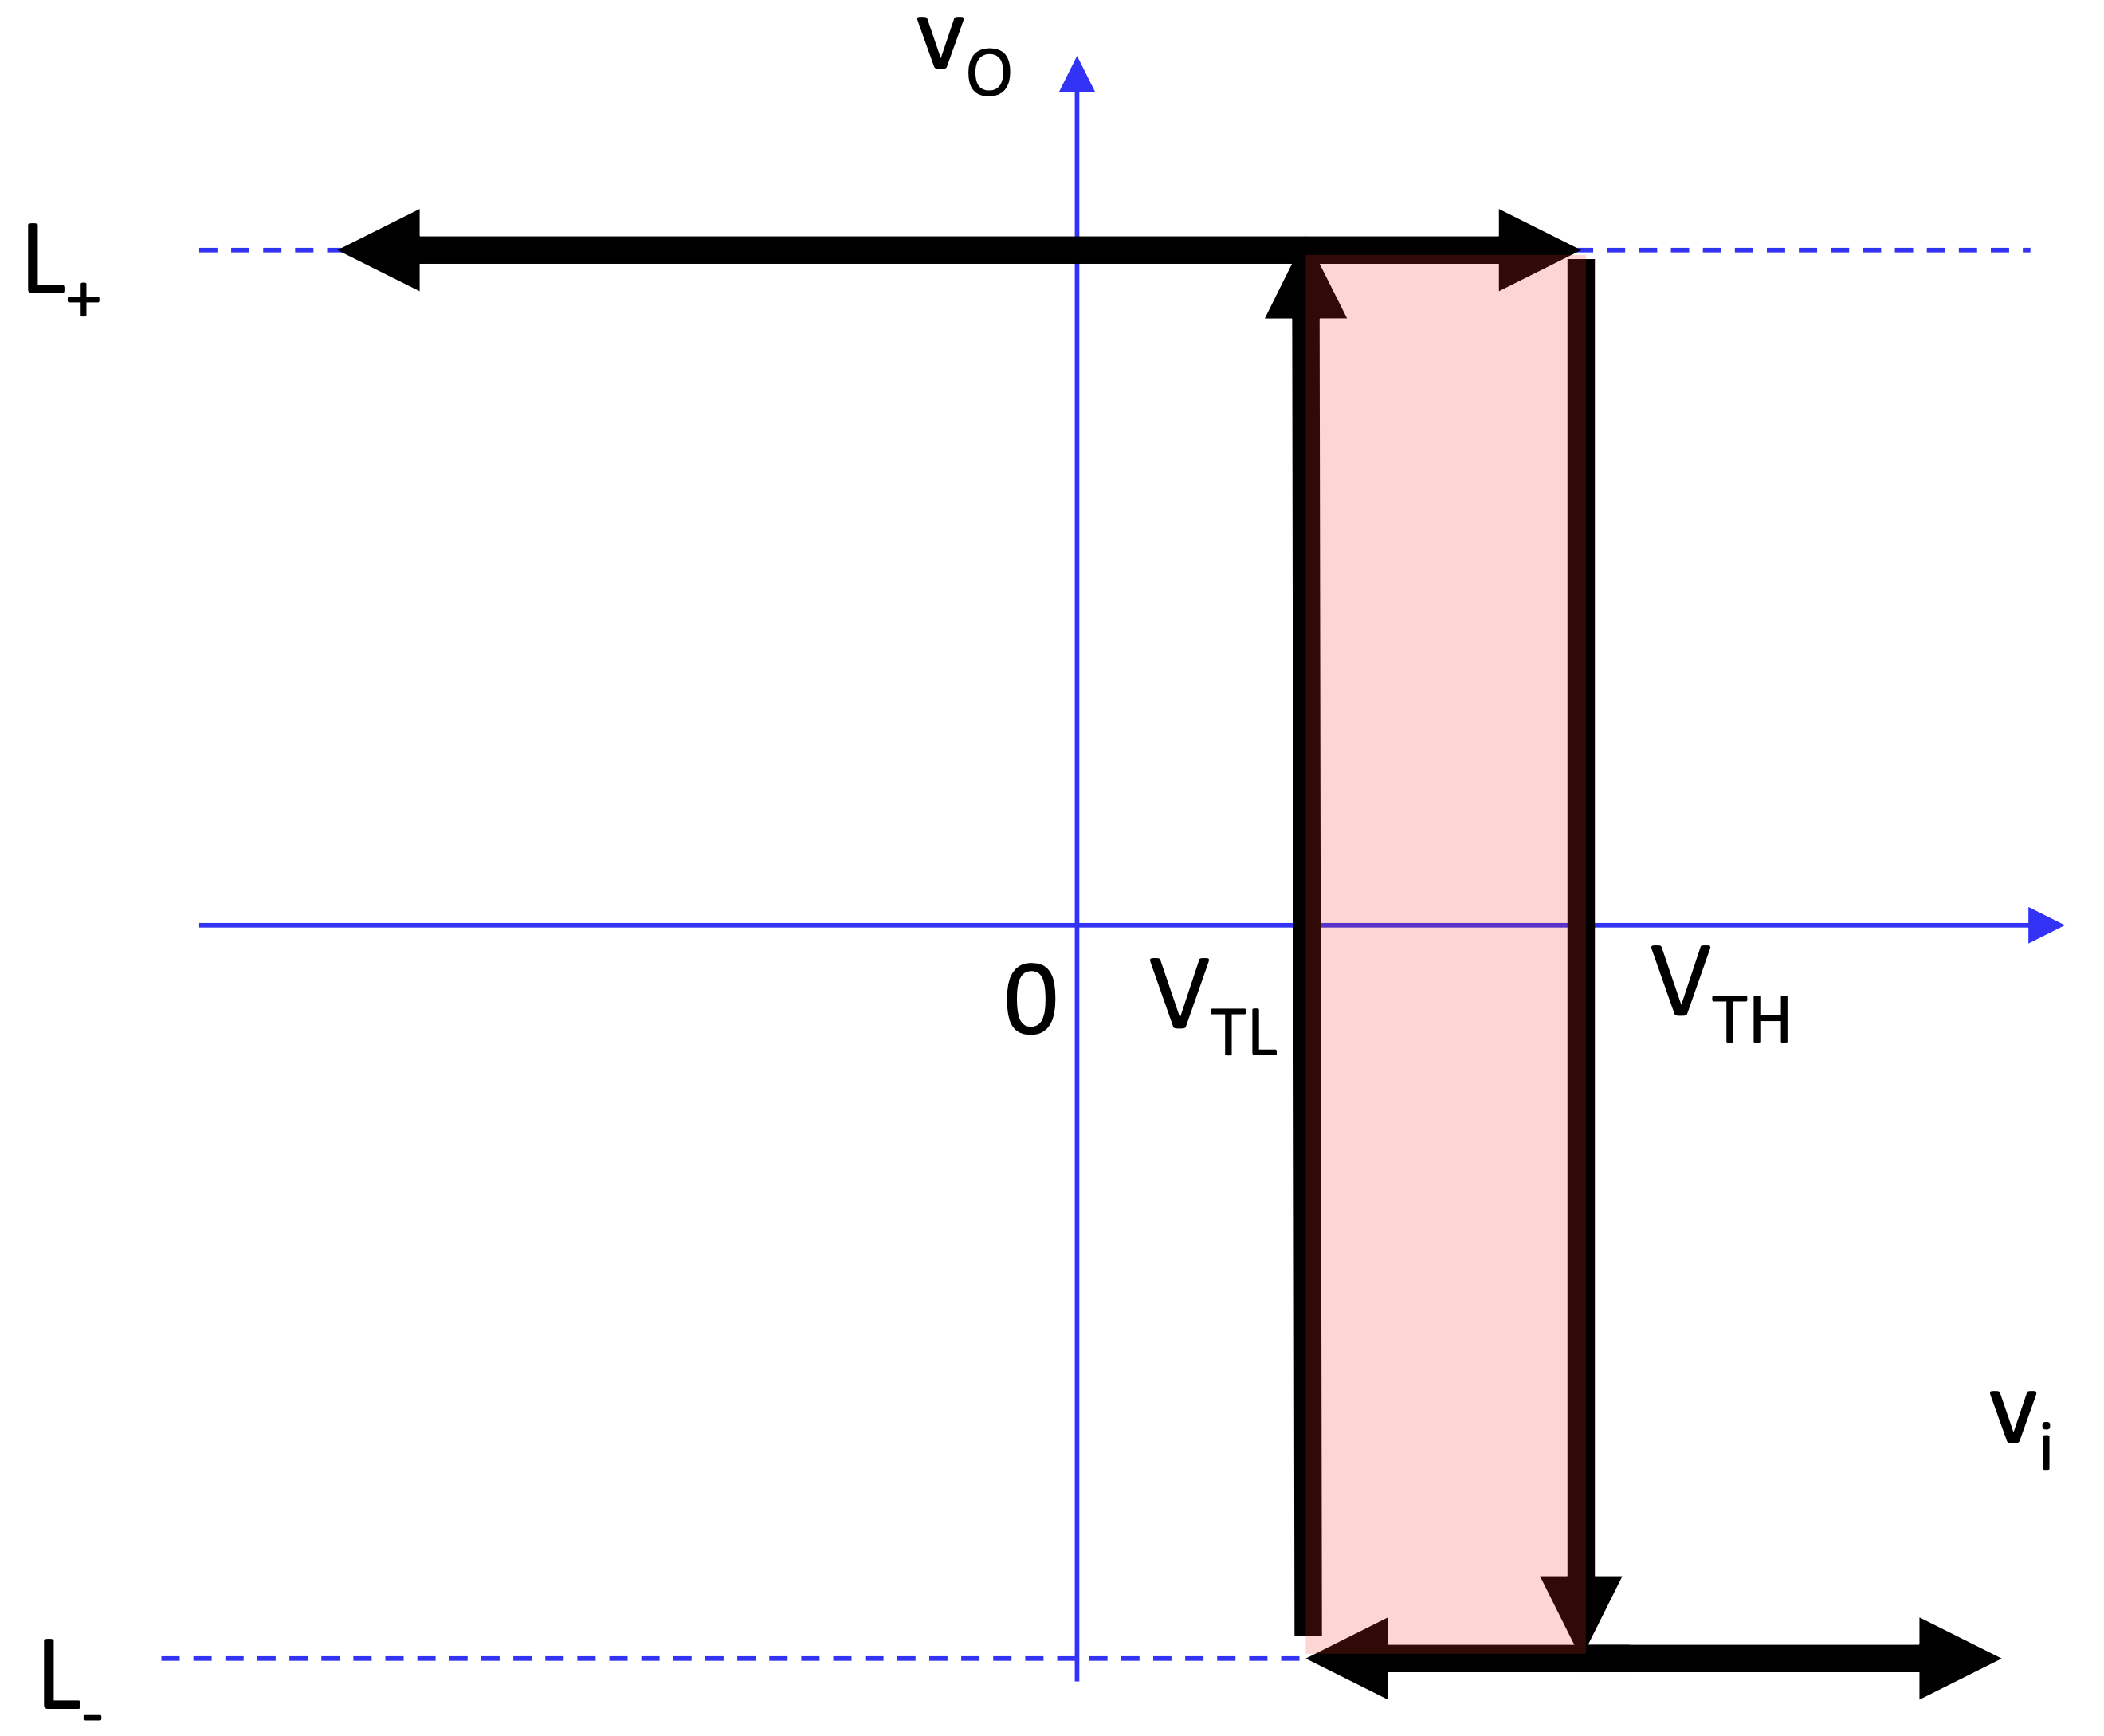
\includegraphics[width=0.7\textwidth]{immagini/inverting_bistable_offset.png}
	\end{minipage}
\end{center}

\subsubsection*{Fixed output voltage}
Saturation output voltages \(L_+\) and \(L_-\) of the op amp are not always defined and depend on the specific op amp used.
To fix the output voltage to a defined value, we can add two zener diodes face-to-face between output and ground. There is
also a resistor to bias the zener diodes and control the current through them.

Alternatively, we can use a 4-diode rectifier bridge to keep the zener diode in the correct orientation regardless of the
output voltage polarity.

\begin{center}
	\begin{minipage}{0.45\textwidth}
		\vspace{0.7cm}
		\centering \begin{circuitikz}[american, scale=0.8, transform shape]
			\ctikzset{diodes/scale=0.8}
			\draw (0,0) node[op amp, yscale=-1] (opamp) {};
			\node[ground] at (opamp.-) {}; 
			\node[left] at (opamp.+) {\(V_+\)};
			\draw (opamp.+) -- ++(0,1);
			\draw (opamp.out) to[R, l=\(R\)] ++(1.5,0) to[short, -o] ++(0.5,0) node[right] {\(V_{out}\)};
			\draw (opamp.out) ++(1.5,0) -- ++(0, 1.5) -- ++(-1.5,0)
			to[R, l=\(R_2\)] ++(-2.5, 0)
			to[R, l=\(R_1\)] ++(-2, 0) -- ++(-0.2,0)
			to[vsource, l_=\(V_{in}\)] ++(0, -1.5) ++(0, 0.3) node[ground] {};
			\draw (opamp.out) ++(1.5,0)
			to[zzDo] ++(0, -1.5) ++(0,-1.2)
			to[zzDo] ++(0, 1.5) ++(0,-1.1) node[ground] {};
		\end{circuitikz} \\[5pt]
		\footnotesize Bistable circuit with fixed output voltage using two zener diodes
	\end{minipage}
	\begin{minipage}{0.45\textwidth}
		\centering \begin{circuitikz}[american, scale=0.8, transform shape]
			\ctikzset{diodes/scale=0.8}
			\draw (0,0) node[op amp, yscale=-1] (opamp) {};
			\node[ground] at (opamp.-) {}; 
			\node[left] at (opamp.+) {\(V_+\)};
			\draw (opamp.+) -- ++(0,1);
			\draw (opamp.out) to[R, l=\(R\)] ++(1.5,0) to[short, -o] ++(0.5,0) node[right] {\(V_{out}\)};
			\draw (opamp.out) ++(1.5,0) -- ++(0, 1.5) -- ++(-1.5,0)
			to[R, l=\(R_2\)] ++(-2.5, 0)
			to[R, l=\(R_1\)] ++(-2, 0) -- ++(-0.2,0)
			to[vsource, l_=\(V_{in}\)] ++(0, -1.5) ++(0, 0.3) node[ground] {};
			\draw (opamp.out) ++(1.5,0) -- ++(0,-0.5) node (StartNode) {};

			\coordinate (DCplus)  at (StartNode);
			\coordinate (AC1)     at ([xshift=-1.4cm, yshift=-1.4cm]DCplus);
			\coordinate (DCminus) at ([xshift=1.4cm, yshift=-1.4cm]AC1);
			\coordinate (AC2)     at ([xshift=2.8cm, yshift=0cm]AC1);

			\draw (AC1) to[D] (DCplus); 
			\draw (AC1) to[D] (DCminus);
			\draw (DCminus) to[D] (AC2);
			\draw (DCplus) to[D] (AC2);
			\draw (AC1) to[zzDo] (AC2);
			\node[ground] at (DCminus) {};
		\end{circuitikz} \\[5pt]
		\footnotesize Bistable circuit with fixed output voltage using a diode bridge and a zener diode
	\end{minipage}
\end{center}

\newpage

\subsection{Triangular wave generator - Astable multivibrator}
\subsubsection*{Circuit}
Bistable circuits require an external trigger to switch between the two stable states. If we want to generate a periodic signal,
we can create a loop made of a bistable circuit and an integrator. The output of the bistable circuit is a square wave that feeds
the input of the integrator, which produces a triangular wave that feeds back the bistable circuit to switch its state. This
new auto-oscillating circuit is called astable multivibrator. It's important to use a non inverting bistable circuit with an
inverting integrator or vice versa to ensure oscillation.

\begin{center}
	\begin{minipage}{0.6\textwidth}
		\centering \begin{circuitikz}[american, scale=0.8, transform shape]
			\draw (0,0) node[op amp, yscale=-1] (opamp) {};
			\node[ground] at (opamp.-) {};
			\draw (opamp.out) to[short, -o] ++(0.5,0) node[right] {\(V_{out2}\)};
			\draw (opamp.out) node[circ] {} -- ++(0, 1.5)
				to[R, l=\(R_2\)] ++(-2.38, 0) -- (opamp.+);
			
			\draw (-5,0) node[op amp, yscale=-1] (opamp2) {};
			\draw (opamp2.+) -- ++(-0.5,0) node[ground] {};
			\draw (opamp2.out) to[short, -o] ++(0, 1) node[above] {\(V_{out1}\)};
			\draw (opamp2.out) -- ++(0, -1.5)
				to[C, name=c] ++(-2.38, 0);
			\draw (opamp.+) to[R, l=\(R_1\)] ++(-2, 0) to[short] (opamp2.out) node[circ] {};
			\draw (opamp2.-) -- ++(0, -2.5) to[R, name=r, i<=$I_R$] ++(2.38,0) -- ++(5,0) -- (opamp.out);

			\node at (c) [xshift=0.4cm, yshift=0.3cm, inner sep=1pt] {\(C\)};
			\node at (c) [xshift=0.7cm, yshift=-0.3cm, inner sep=1pt] (cminus) {\(-\)};
			\node at (c) [xshift=-0.7cm, yshift=-0.3cm, inner sep=1pt] (cplus) {\(+\)};
			\node at (r) [xshift=0.6cm, yshift=0.3cm, inner sep=1pt] {\(R\)};

			\draw[-{Latex}]
				($(cminus) + (-0.1, -0.2)$) to[out=-110, in=-70] 
				node[pos=0.5, fill=white, inner sep=1pt] {$V_C$} 
				($(cplus) + (0.1, -0.2)$);
		\end{circuitikz}
	\end{minipage}
	\begin{minipage}{0.35\textwidth}
		\centering 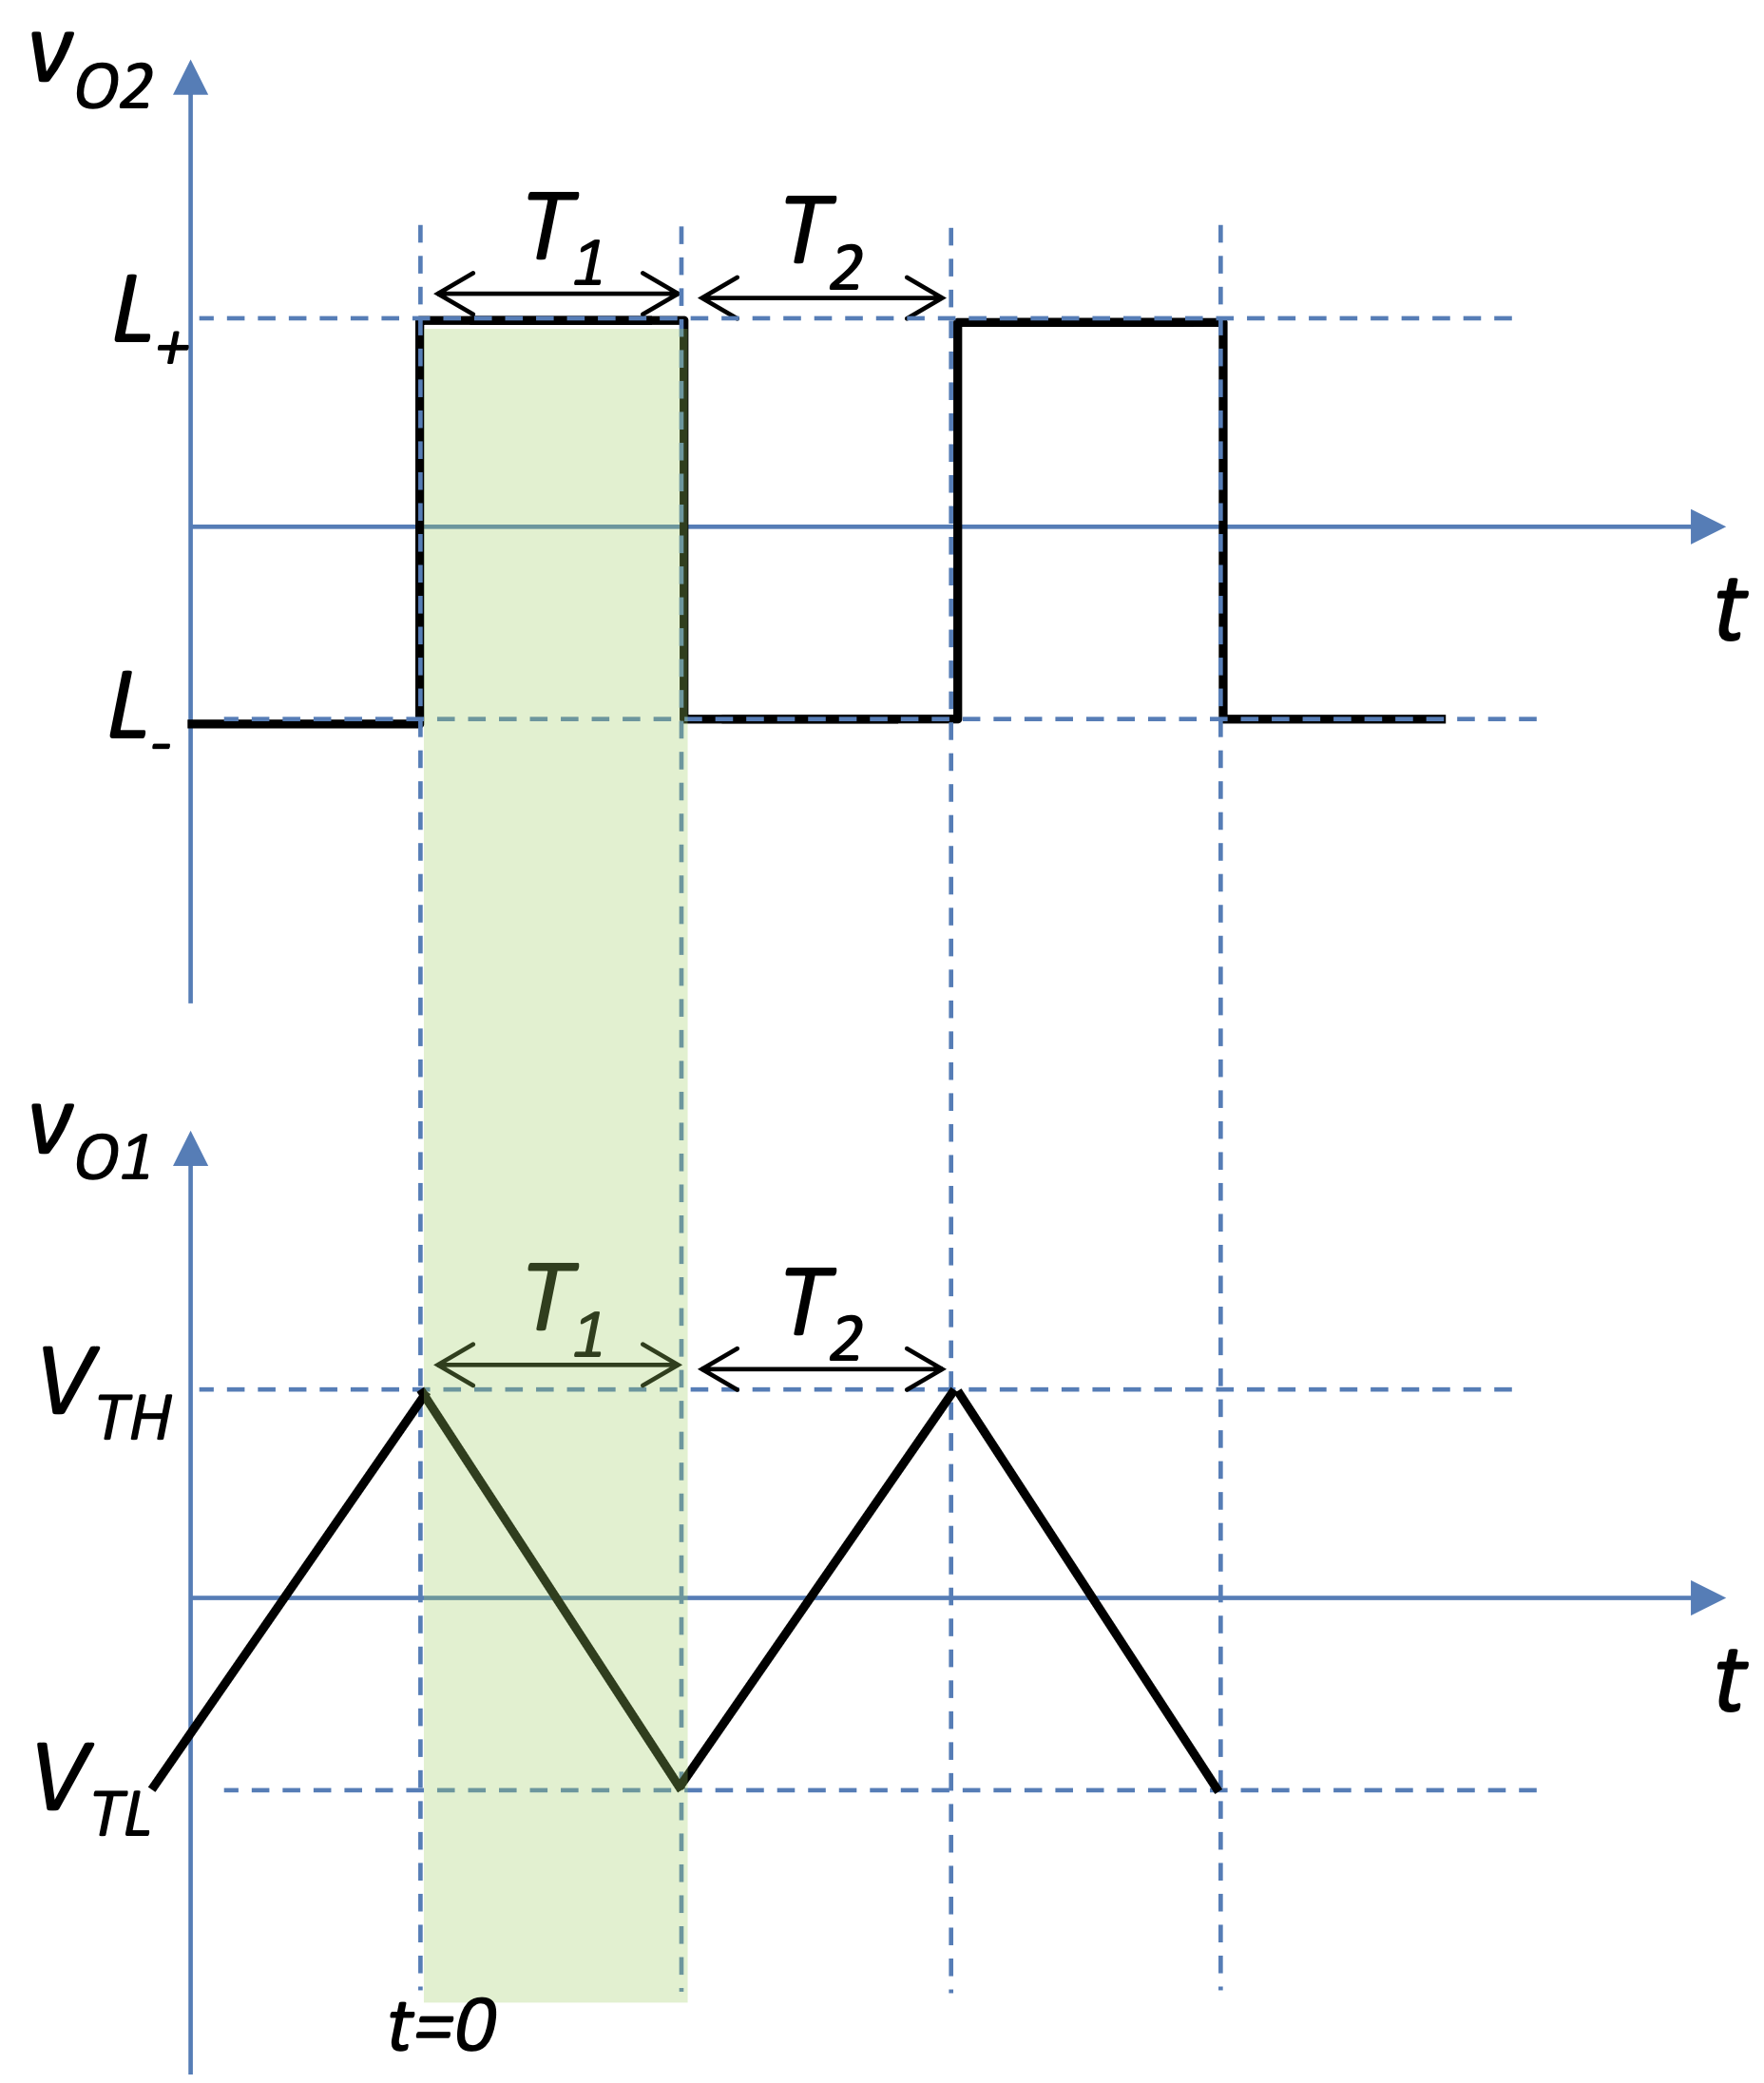
\includegraphics[width=0.8\textwidth]{immagini/astable_multivibrator.png}
	\end{minipage}
\end{center}

\subsubsection*{Circuit behaviour}
When \(V_{out2}\) is at \(L_+\), there is a constant current \(I_R = L_+ / R\) through the resistor \(R\) that discarge the
capacitor \(C\) at a constant rate of \(\frac{L_+}{RC}\). The output voltage \(V_{out1}\) decreases linearly with time, as
given by the following reasoning:
\[I_C = C \frac{dV_C}{dt} = - C \frac{dV_{out1}}{dt} = \frac{L_+}{R} \;\; \rightarrow \;\; V_{out1}(t) = V_{out1}(0) - \int \frac{L_+}{R} dt = V_{out1}(0) - \frac{L_+}{RC} t\]
When the output voltage \(V_{out1}\) reaches the negative threshold voltage \(V_{TL}\) of the bistable circuit, the output
voltage \(V_{out2}\) switches to \(L_-\) and the current through the resistor \(R\) becomes \(I_R = L_- / R\) (and changes sign).
The capacitor starts charging at a constant rate of \(\frac{L_-}{RC}\) and the output voltage \(V_{out1}\) increases linearly
until it reaches the positive threshold voltage \(V_{TH}\) of the bistable circuit that changes the output voltage \(V_{out2}\)
back to \(L_+\) and the cycle repeats indefinitely.

The period of the output signals is the time it takes for the output voltage \(V_{out1}\) to go from \(V_{TH}\) to \(V_{TL}\)
and back to \(V_{TH}\):
\begin{align*}
	\text{in } T_1, \; V_{out1} \text{ goes from } V_{TH} \text{ to } V_{TL}: \quad &\frac{V_{TH} - V_{TL}}{T_1} = \frac{L_+}{RC} \quad \rightarrow \quad T_1 = RC \frac{(V_{TH} - V_{TL})}{L_+} \\
	\text{in } T_2, \; V_{out1} \text{ goes from } V_{TL} \text{ to } V_{TH}: \quad &\frac{V_{TL} - V_{TH}}{T_2} = \frac{L_-}{RC} \quad \rightarrow \quad T_2 = RC \frac{(V_{TL} - V_{TH})}{L_-}
\end{align*}
If the bistable circuit is symmetric, with \(L_+ = L_-\), then the total period of the output signals is:
\[T = T_1 + T_2 = RC \frac{(V_{TH} - V_{TL})}{L_+} + RC \frac{(V_{TL} - V_{TH})}{L_-} = 2 RC \frac{(V_{TH} - V_{TL})}{L_+}\]

\newpage

\subsection{Sine wave generator}
By adding a bandpass filter to the triangular wave signal from the output of the astable multivibrator, it is possible to
attenuate the harmonics of the signal and keep the fundamental sine wave. The bandpass filter can be a first-order low-pass
filter implemented with an op amp. A first order low-pass filter may not be enough to obtain a good sine wave, because the third harmonic is
attenuated to 30\%, maybe a second order low-pass filter is needed.

\begin{center}
	\begin{minipage}{0.8\textwidth}
		\centering \begin{circuitikz}[american, scale=0.8, transform shape]
			\draw (0,0) node[op amp, yscale=-1] (opamp) {};
			\node[ground] at (opamp.-) {};
			\draw (opamp.out) to[short, -o] ++(0.5,0) node[right] {\(V_{out2}\)};
			\draw (opamp.out) node[circ] {} -- ++(0, 1.5)
				to[R, l=\(R_2\)] ++(-2.38, 0) -- (opamp.+);
			
			\draw (-5,0) node[op amp, yscale=-1] (opamp2) {};
			\draw (opamp2.+) -- ++(-0.5,0) node[ground] {};
			\draw (opamp2.out) to[short, -o] ++(0, 1) node[above] {\(V_{out1}\)};
			\draw (opamp2.out) -- ++(0, -1.5)
				to[C, name=c] ++(-2.38, 0);
			\draw (opamp.+) to[R, l=\(R_1\)] ++(-2, 0) to[short] (opamp2.out) node[circ] {};
			\draw (opamp2.-) -- ++(0, -2) to[R, name=r] ++(2.38,0) -- ++(5,0) -- (opamp.out);

			\node at (c) [xshift=0.4cm, yshift=0.3cm, inner sep=1pt] {\(C\)};
			\node at (r) [xshift=0.6cm, yshift=0.3cm, inner sep=1pt] {\(R\)};

			\draw (6,0) node [op amp] (opamp3) {};
			\draw (opamp3.+) node[ground] {};
			\draw (opamp3.out) to[short, -o] ++(0.5,0) node[right] {\(V_{out3}\)};
			\draw (opamp3.out) -- ++(0, 1.5)
				to[C, name=c4] ++(-2.38, 0) -- (opamp3.-);
			\draw (opamp3.out) -- ++(0, 2.5)
				to[R, name=r4] ++(-2.38, 0) -- (opamp3.-);
			\draw (opamp3.-) to[R, l=\(R_3\)] ++(-2, 0) -- ++(-1,2) to[short] ++(-4.4,0) to[short] (opamp2.out);
			
			\node at (c4) [xshift=0.4cm, yshift=0.3cm, inner sep=1pt] {\(C_4\)};
			\node at (r4) [xshift=0.6cm, yshift=0.3cm, inner sep=1pt] {\(R_4\)};
		\end{circuitikz}
	\end{minipage}
\end{center}

The trasnfer characteristic of the low-pass filter is given by:
\[H(j\omega) = \frac{V_{out3}}{V_{in3}} = -\frac{Z_f}{Z_{in}} = - \frac{R_4 \cdot Z_{C4}}{R_4 + Z_{C4}} \cdot \frac{1}{R_3} = - \frac{R_4 / j\omega C_4}{R_4 + 1 / j\omega C_4} \cdot \frac{1}{R_3} = \underbrace{- \frac{R_4}{R_3}}_{\text{\footnotesize gain}} \cdot \underbrace{\frac{1}{1 + j\omega R_4 C_4}}_{\text{\footnotesize low-pass filter}}\]
\[\left|H(j\omega)\right| = \left|\cdot \frac{1}{\sqrt{1 + (\omega R_4 C_4)^2}}\right| = \frac{1}{\sqrt{2}} \quad \rightarrow \quad \omega = \frac{1}{R_4 C_4} \quad \rightarrow \quad f_c = \frac{1}{2\pi R_4 C_4}\]
